\documentclass[11pt]{article}
\usepackage[margin=1in]{geometry} 
\usepackage[T1]{fontenc}
\usepackage{graphicx}
\newcommand\tab[1][1cm]{\hspace*{#1}}

\title{CS483 Project Proposal Template\\
\large Team One}

\author{
  Clara, Alberto      \texttt{- alberto.clara@wsu.edu}
  \and
  AlSarhi, Saeed      \texttt{- saeed.alsarhi@wsu.edu}
  \and
  Wellington, Patrick      \texttt{- patrick.wellington@wsu.edu}
}
\date{10/26/2018}

\begin{document}

\maketitle
\section{Team Name}
TEAM ONE

\section{Members}
Alberto Clara
Saeed AlSarh
Patrick Wellington

\section{Database Schema}
Movie(Name, Year\_of\_release, Description, Rating, Genre, IMDB\_Url, Votes\_Count)\newline
The Data Set size is around 5,000 tuples. \newline
\text{
schema = Schema( \newline
    \tab Name = ID(stored=True), \newline
    \tab Year\_of\_release = TEXT(stored=True), \newline
    \tab Description = TEXT(stored=True), \newline
    \tab Rating = TEXT(stored=True), \newline
    \tab Genre = TEXT(stored=True), \newline
    \tab IMDB\_URL = TEXT(stored=True), \newline
    \tab Votes\_Count = TEXT(stored=True), \newline
)
}

\section{Size of Database}
5,000 tuples

\section{Five examples of searches and the top 10 tuples returned for each}
Example 1: Man \newline
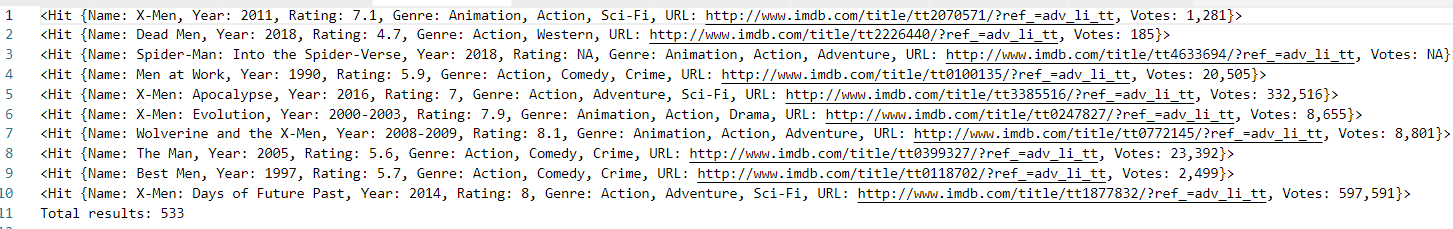
\includegraphics[width=170mm,scale=0.5]{Assignment3Ex1.png}\newline
Example 2: Spider \newline
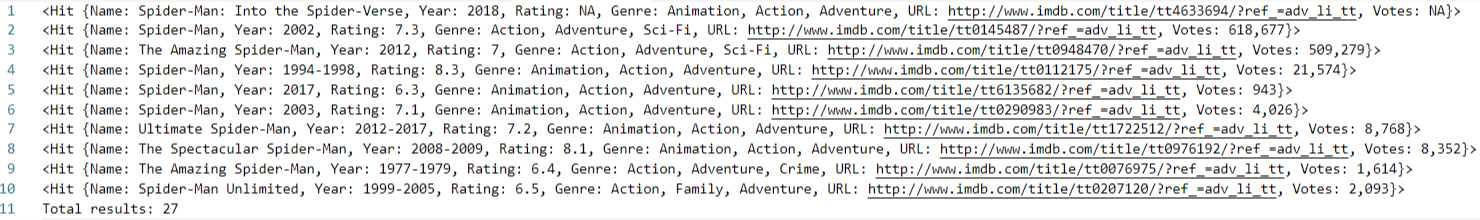
\includegraphics[width=170mm,scale=0.5]{Assignment3Ex2.png}\newline
Example 3: Rain \newline
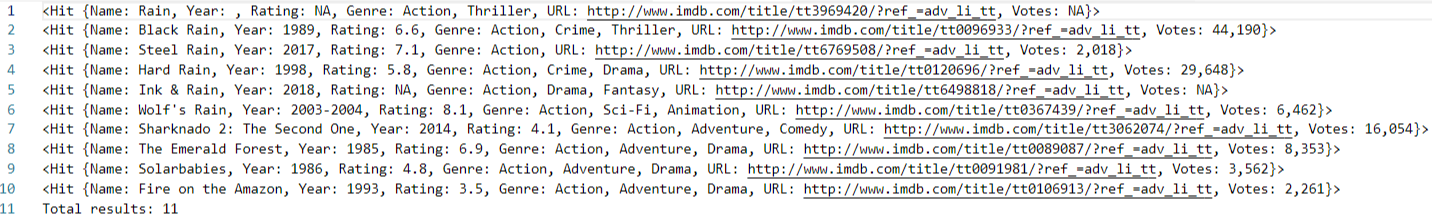
\includegraphics[width=170mm,scale=0.5]{Assignment3Ex3.png}\newline
Example 4: Dark \newline
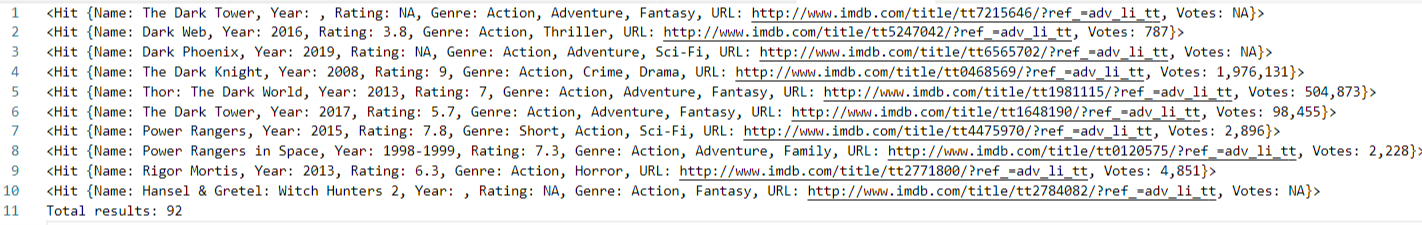
\includegraphics[width=170mm,scale=0.5]{Assignment3Ex4.png}\newline
Example 5: Hero \newline
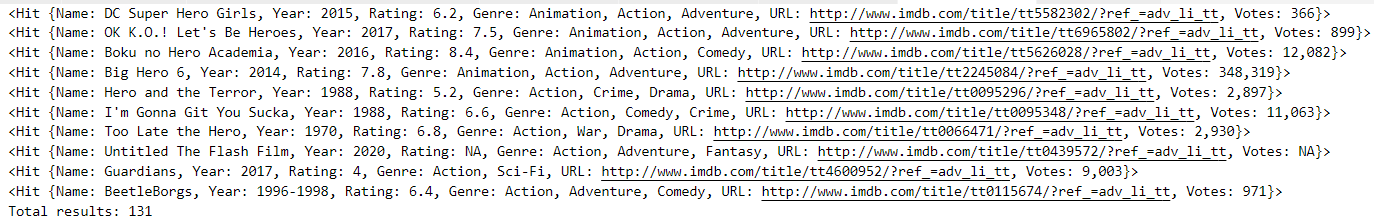
\includegraphics[width=170mm,scale=0.5]{Assignment3Ex5.png}\newline

%\bibliographystyle{ieeetr}
%\bibliography{bib.bib}
\end{document}
